\chapter{Aspectos relevantes del desarrollo}
En este apartado se explicarán los experimetos realizados y las conclusiones obtenidas a lo largo de estos.

\section{Obtención de los datos de prueba}\label{sect:datosPrueba}
Como se ha comentado previamente los datos se obtienen del proyecto \textit{``AI4Boundaries: an open AI-ready dataset to map field boundaries with Sentinel-2 and aerial photography''} \cite{AI4boundaries}, concretamente del  \href{https://jeodpp.jrc.ec.europa.eu/ftp/jrc-opendata/DRLL/AI4BOUNDARIES/}{repositorio de datos} del proyecto.

Como podemos ver se organizan en varias 3 carpetas:

\begin{itemize}
	\item{Orthophotos}: Carpeta dónde aparecen las Ortofotos del proyecto. Estas no son utilizadas en este proyecto.
	\item{Sampling}: Carpeta dónde se almacenan los csv que relacionan las distintas imágenes con su respectiva url en el ftp sobre el repositorio, tanto la imagen en formato .nc como las máscaras de capa .tif. Esta carpeta tampoco se ha utilizado ya que las imágenes se han descargado para las pruebas en lugar de hacer una carga dinámica.
	\item{Sentinel2}: Carpeta que guarda tanto las imágenes como las máscaras además de archivos csv que muestran cuantos píxeles de cada tipo tienen los resultados.
\end{itemize}

Por la cantidad de datos y los recursos de los que dispone el sistema se ha decidido trabajar solo con un subconjunto de los datos, concretamente los correspondientes a 128 imágenes de España.

\section{Visualización de los datos y composición de la imagen}
Lo primero que se realizó fue una exploración de los datos, para comprender mejor estos y ver sus estructuras, para eso se extrajeron las bandas 4, 3 y 2, correspondientes a la banda Roja, Verde y Azul, se visualizaron en como podemos ver en la figura ~\ref{fig:bandas_rgb} y posteriormente se compusieron en una imágen RGB como podemos ver en la figura ~\ref{fig:imagen_compuesta}.

\begin{figure}[H]
	\centering
	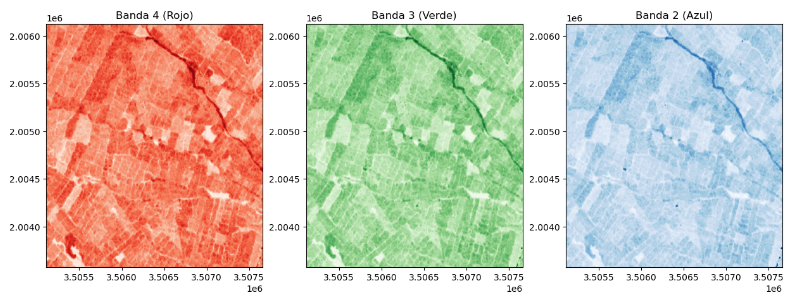
\includegraphics[width=1\textwidth]{Bandas_RGB_separadas}
	\caption[Visualización de las Bandas RGB separadas]{Visualización de las Bandas RGB separadas.}
	\label{fig:bandas_rgb}
\end{figure}

\begin{figure}[H]
	\centering
	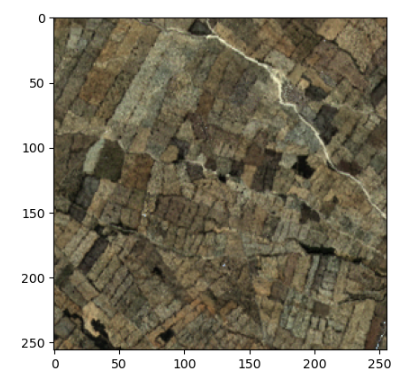
\includegraphics[width=0.4\textwidth]{Imagen_compuesta}
	\caption[Visualización de la imagen compuesta con las bandas RGB]{Visualización de la imagen compuesta con las bandas RGB.}
	\label{fig:imagen_compuesta}
\end{figure}

Una vez visualizada la imagen se comprobó cómo son las máscaras de capa, estas tienen 4 capas distintas la máscara de capa, una mascara de límites,una mascara de distancia y una enumeración de campos. Se ha decidido entrenar los modelos con la primera opción. Como podemos ver en la figura ~\ref{fig:mascara_sola}.

\begin{figure}[H]
	\centering
	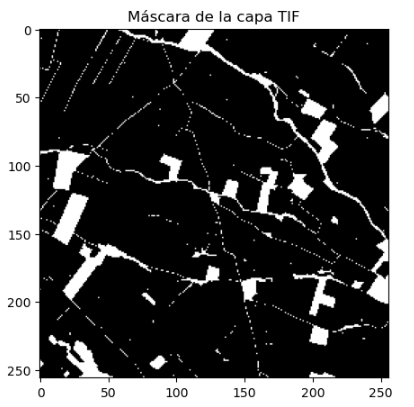
\includegraphics[width=0.66\textwidth]{Mascara_tif}
	\caption[Visualización de la máscara de capa de las delimitaciones]{Visualización de la máscara de capa de las delimitaciones.}
	\label{fig:mascara_sola}
\end{figure}

Tras eso se superpuso la capa con la imagen para comprobar cuánto se adecua con la imagen. Como se puede ver en la figura  ~\ref{fig:mascara_superpuesta} registran los grandes límites.

\begin{figure}
	\centering
	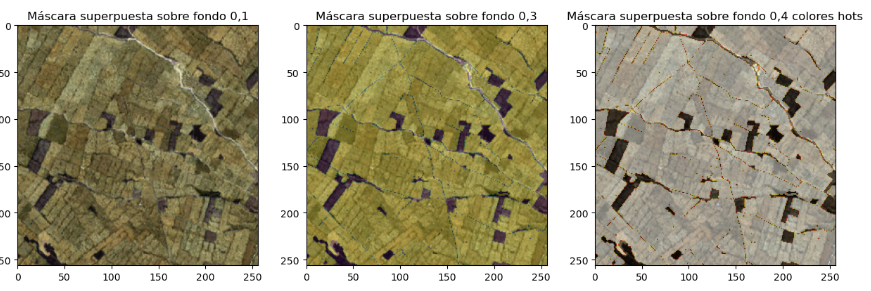
\includegraphics[width=1\textwidth]{Mascara_superpuesta}
	\caption[Visualización de la máscara de capa superpuesta con la imagen]{Visualización de la máscara de capa superpuesta con la imagen.}
	\label{fig:mascara_superpuesta}
\end{figure}

 
\section{Modelos sin contexto}
En este apartado intentaremos entrenar tres modelos: KNN, SVM y RandomForest. Estos no tienen en cuenta el contexto de los píxeles, predicen unicamente en base a la información de cada píxel por lo que se asumía, cosa que se comprobó que obtienen unos resultados peores. 

\subsection{KNN}
Se empezó por KNN, este tuvo un tiempo de entrenamiento de 57.88 segundos. Se hizo una predicción sobre la imagen del inicio para poder visualizar el resultado. Los resultados son la figura ~\ref{fig:prediccion_knn}.

\begin{figure}[H]
	\centering
	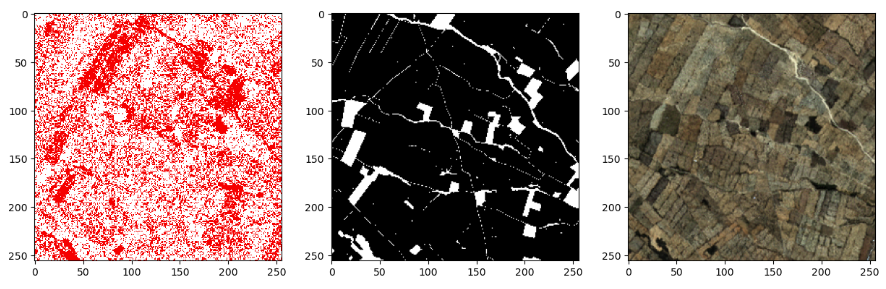
\includegraphics[width=1\textwidth]{Clasificacion_KNN}
	\caption[Visualización de la predicción sobre la imagen KNN]{Visualización de la predicción sobre la imagen por el modelo KNN comparada con el resultado previsto y la imagen orginal.}
	\label{fig:prediccion_knn}
\end{figure}

\begin{figure}[H]
	\centering
	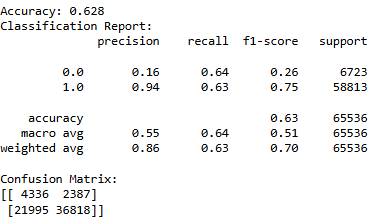
\includegraphics[width=0.66\textwidth]{Metricas_KNN}
	\caption[Métricas obtenidas para el modelo KNN]{Métricas obtenidas para el modelo KNN.}
	\label{fig:metricas_knn}
\end{figure}

Las métricas obtenidas por el modelo han sido las mostradas en la figura ~\ref{fig:metricas_knn}. 
Si se analizan los resultados podemos ver que si bien reconoce algunas estructuras y se puede llegar a intuir la imagen en la predicción, hay mucho ruido en la imagen y probablemente el hecho de que haya obtenido unos resultados es derivado de que es un conjunto de datos relativamente desbalanceado.

\subsection{SVM}
El siguiente modelo a probar es SVM, el cual no se pudo llegar a entrenar ya que el tiempo que requirió  para entrenarse era claramente excesivo superando las 16 horas antes de que se decidiera pararlo.

\subsection{Random Forest}
Finalmente Se probó Random Forest, el cual se lanzo con todos los núcleos posibles en paralelo, de cara a mejorar su eficiencia. igualmente tuvo un tiempo de entrenamiento de 1273.35 segundos. Se pueden ver los resultados de la predicción en la figura ~\ref{fig:prediccion_rf} y las métricas ~\ref{fig:metricas_rf}.


\begin{figure}[H]
	\centering
	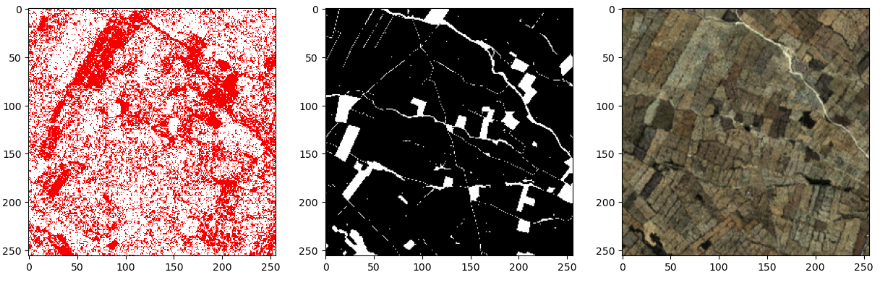
\includegraphics[width=1\textwidth]{Clasificacion_Random_Forest}
	\caption[Visualización de la predicción sobre la imagen Random Forest]{Visualización de la predicción sobre la imagen por el modelo Random Forest comparada con el resultado previsto y la imagen orginal.}
	\label{fig:prediccion_rf}
\end{figure}

\begin{figure}[H]
	\centering
	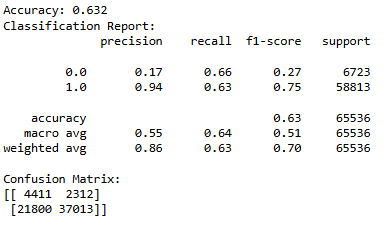
\includegraphics[width=0.66\textwidth]{Metricas_Random_Forest}
	\caption[Métricas obtenidas para el modelo Random Forest]{Métricas obtenidas para el modelo Random Forest.}
	\label{fig:metricas_rf}
\end{figure}

\section{Modelo U-Net}
Finalmente el grueso de las pruebas se hicieron son las relacionadas con la red convolucional de tipo U-Net. Esta como ya se ha mentado tiene contexto de los píxeles alrededor del que se está analizando. Esto de manera teórica se supone que obtendrá mejores resultados, cosa que se ha probado.

Se empezó por implementar la red neuronal, siguiendo los pasos del paper \cite{Unet} aunque se implementó una segunda versión en la cual hay Dropout en tre las convoluciones de una misma capa, para evitar el sobreajuste.

En todas las opciones se escogió como optimizador adam, como métricas accuracy y como función de perdida binary\_crossentropy. Estos han tenido un tiempo de entrenamiento por época de entre 250 y 300 segundos. Marcando un accuracy según las métricas de Keras de entre 0.75 y 0.86 siendo a partir de 10 épocas normalmente superiores a 0.8.

De cara a buscar cual es la mejor configuración posible se probaron en un inicio 8 modelos, los cuales se hizo una predicción sobre la imagen previa para visualmente analizar cual ha sido más adecuado. Se muestra en la figura ~\ref{fig:predicciones}.

\begin{figure}
	\centering
	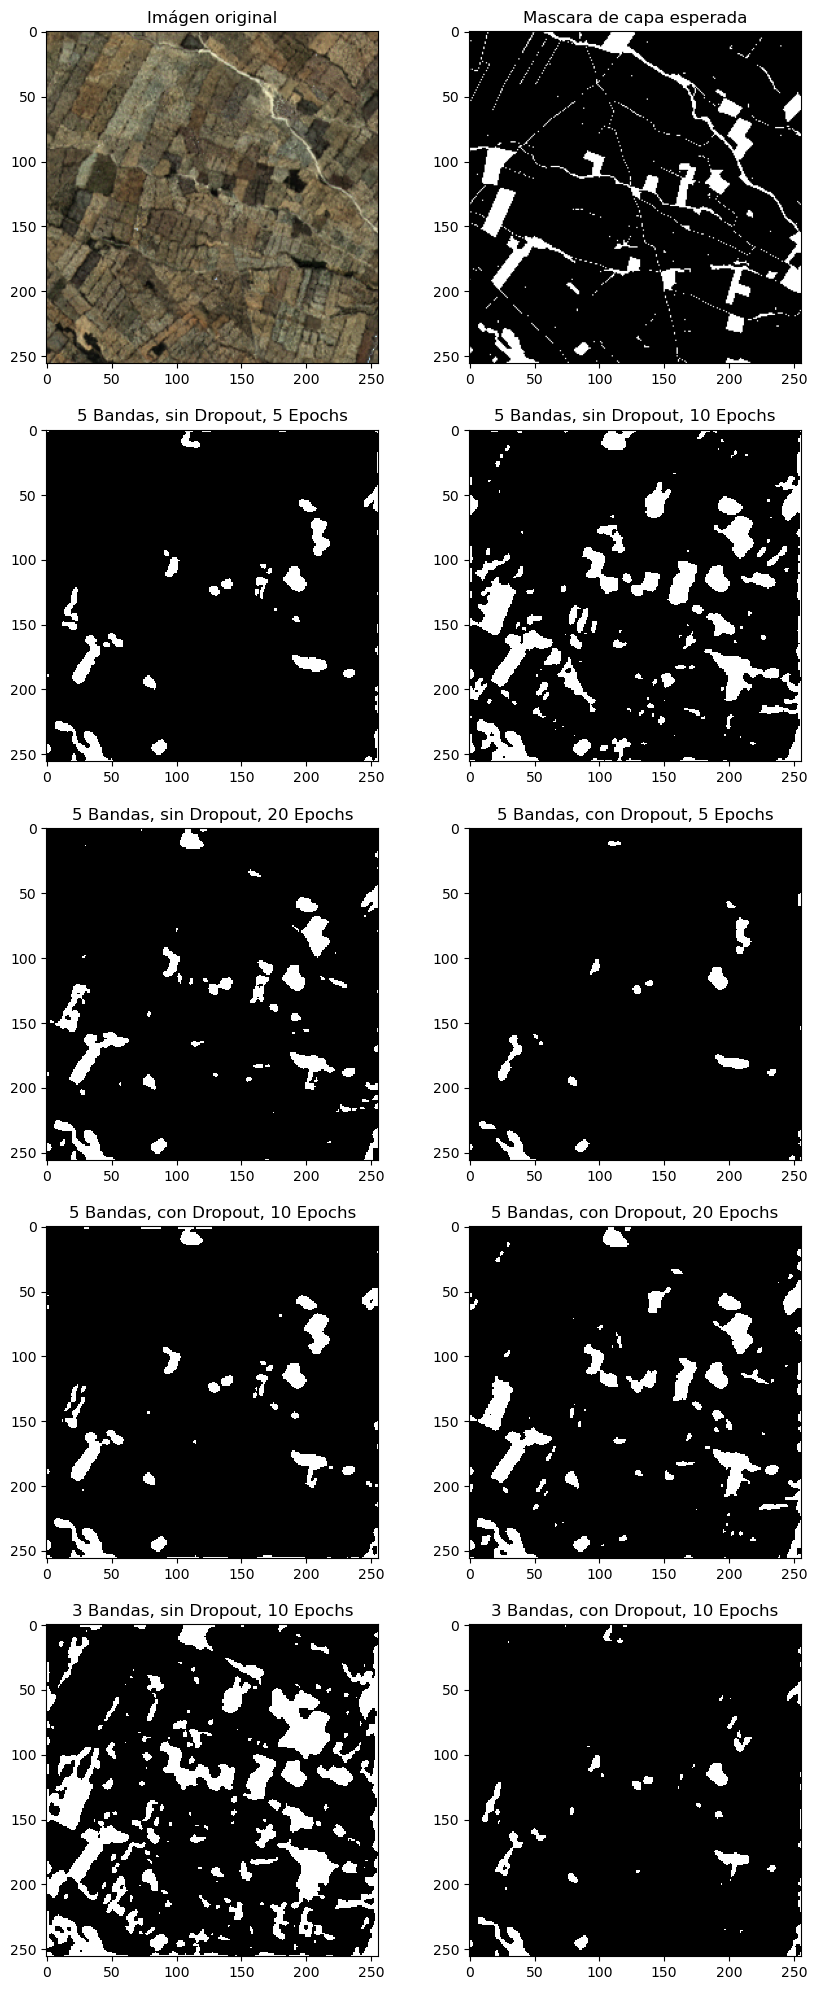
\includegraphics[scale=0.4]{resultados_unet}
	\caption[Predicciones realizadas por los modelos descritos]{Predicciones realizadas por los modelos descritos.}
	\label{fig:predicciones}
\end{figure}

Finalmente viendo los resultados dados se decidió entrena un modelo más esta vez con 40 épocas y con dropout, que será el modelo a utilizar.
Los resultados de este lo podemos ver en la figura ~\ref{fig:prediccion_540c}.
	
\begin{figure}[H]
	\centering
	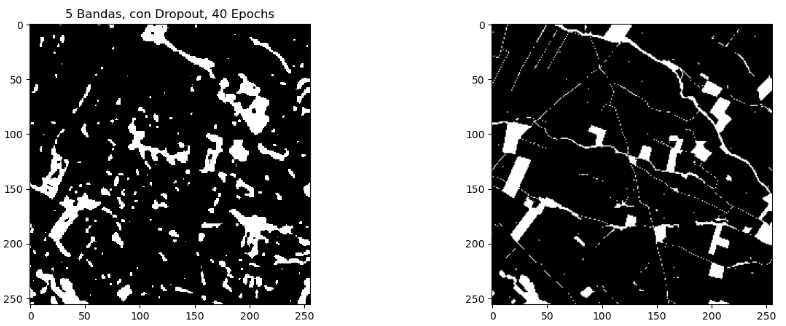
\includegraphics[width=1\textwidth]{Unet_clasificacion_5_bandas_40_epocas_con_dropout}
	\caption[Predicción realizada por el modelo final]{Predicción realizada por el modelo final.}
	\label{fig:prediccion_540c}
\end{figure}

Es reseñable que si bien este muestra esa predicción con un umbral de predicción de 0.5, entendiendo que este es el punto a partir del cual en la predicción se considera 1. La predicción sin hacer ese filtrado por umbral muestra una imagen muy interesante que puede ser más interpretable como se puede ver en la figura ~\ref{fig:prediccion_sin_umbral}.
	
\begin{figure}[H]
	\centering
	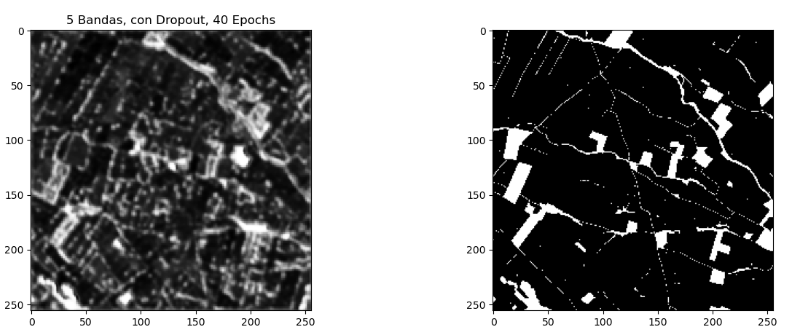
\includegraphics[width=1\textwidth]{Unet_clasificacion_5_bandas_40_epocas_con_dropout_sin_threshold}
	\caption[Predicción realizada por el modelo final sin binarizar]{Predicción realizada por el modelo final sin binarizar.}
	\label{fig:prediccion_sin_umbral}
\end{figure}

Finalmente se evaluaron los modelos y el que mejores métricas consiguió fue el último, tal y como se había predicho. Este tienes las métricas mostradas en la siguiente figura  ~\ref{fig:metricas_u-net}.

\begin{figure}[H]
	\centering
	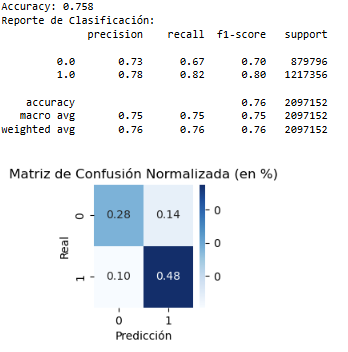
\includegraphics[width=1\textwidth]{metricas_u-net}
	\caption[Métricas del modelo U-Net con 40 Epochs]{Métricas del modelo U-Net con 40 Epochs con dropout.}
	\label{fig:metricas_u-net}
\end{figure}

Analizando estos resultados se puede reseñar que se han obtenido un modelo suficientemente adecuado, aunque puede llegar a ser mejorable.